\section{Additional tables and figures}\label{app:tables}

\begin{figure}[h]
\centering
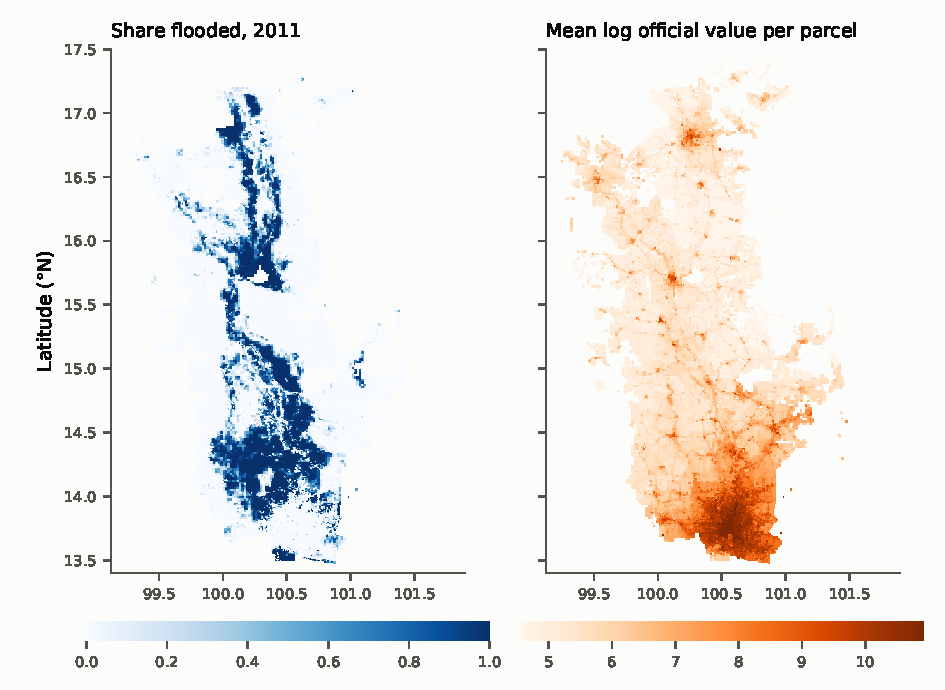
\includegraphics[width=\textwidth]{fig_basin_maps}
\caption{2011 flood share and official land value by cadastral sheet, Chao Phraya basin}
\label{fig:maps}
\tabnote{Each marker is one cadastral sheet (2~km rural, 500~m urban) at its centre. Left: share of the sheet's land pixels flooded in the Global Flood Database event of 5 August 2011 to 9 January 2012 (MODIS, 250~m). Right: mean log official value per parcel, round 2023--26. The near-absence of detected flooding in Bangkok reflects urban under-detection by optical satellites, not an absence of flooding. Sources: Treasury Department official land values, round 2023--26 (snapshot of 2 November 2026); Global Flood Database event DFO~3850 \citep{tellman2021satellite}; author's calculations.}
\end{figure}

\begin{figure}[h]
\centering
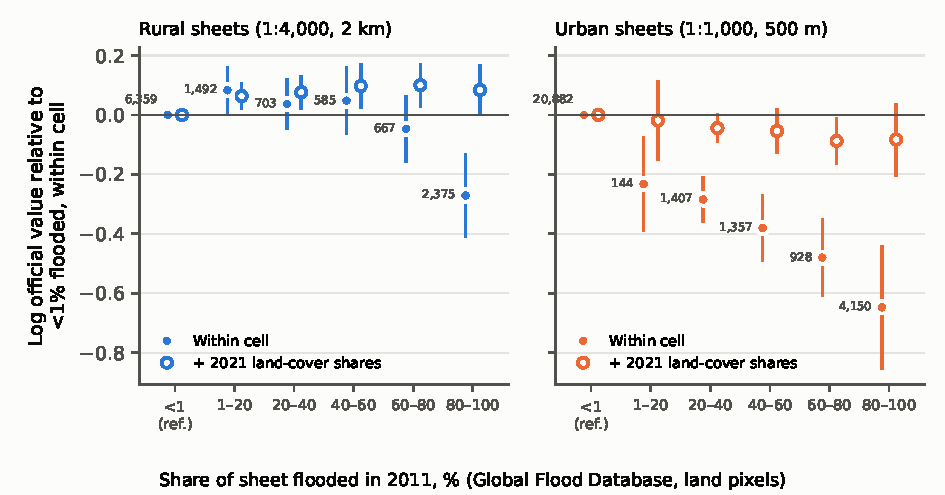
\includegraphics[width=\textwidth]{fig_appraisal_flood_binned}
\caption{Official land value by 2011 flood-share bin, within province, map block and scale}
\label{fig:binned}
\tabnote{Coefficients $\beta_b$ from equation~\eqref{eq:cross} with 95\% intervals (clustered by 1:50,000 block), reference bin $<$1\%. Filled markers: cell effects only; open markers: adding 2021 WorldCover land-cover shares. Numbers are sheets per bin. Table~\ref{tab:binned} gives the estimates.}
\end{figure}

\begin{table}[h]
\centering\footnotesize
\caption{Linear within-cell slopes of official value on 2011 flood share}\label{tab:within}
% Generated by 04_analysis/src/paper_numbers.py. Do not edit.
\begin{adjustbox}{max width=\textwidth}
\begin{tabular}{lccrrr}
\toprule
 & Mean log value & p90 log value & Sheets & Parcels & Clusters \\
\midrule
Rural (1:4,000) & $-$0.488 (0.106) & $-$0.733 (0.148) & 12,181 & 3,700,992 & 108 \\
Urban (1:1,000) & $-$0.650 (0.098) & $-$0.815 (0.110) & 28,868 & 5,074,885 & 95 \\
\bottomrule
\end{tabular}
\end{adjustbox}

\tabnote{Coefficient on the 2011 flood share (0--1) in equation~\eqref{eq:cross} with the share entering linearly and no land-cover controls. Outcomes: parcel-weighted mean and 90th percentile of log official value per \wah\ on the sheet. Standard errors clustered by 1:50,000 block. Source: \texttt{appraisal\_flood\_within.csv}.}
\end{table}

\begin{table}[h]
\centering\footnotesize
\caption{Coarseness of official values within cadastral sheets}\label{tab:discreteness}
% Generated by 04_analysis/src/paper_numbers.py. Do not edit.
\begin{adjustbox}{max width=\textwidth}
\begin{tabular}{lrrrr}
\toprule
Sheet scale & Sheets & Median parcels per sheet & Median distinct values & p90 distinct values \\
\midrule
1:500 & 6,988 & 16 & 2 & 6 \\
1:1,000 & 155,711 & 38 & 5 & 13 \\
1:2,000 & 36,763 & 50 & 7 & 16 \\
1:4,000 & 72,821 & 196 & 11 & 26 \\
\bottomrule
\end{tabular}
\end{adjustbox}

\tabnote{All decoded sheets in the \covProvinces{} provinces, round 2023--26. A ``distinct value'' is a distinct value per \wah\ among the sheet's parcels. Source: \texttt{sheet\_price\_discreteness.csv}.}
\end{table}

\begin{table}[h]
\centering\footnotesize
\caption{2011 flood share by province, Global Flood Database}\label{tab:province2011}
% Generated by 04_analysis/src/paper_numbers.py. Do not edit.
\begin{adjustbox}{max width=\textwidth}
\begin{tabular}{lrrr}
\toprule
Province & Parcels & Share of parcels flooded in 2011 (\%) & Mean GSW occurrence (\%) \\
\midrule
Ayutthaya & 465,874 & 64.6 & 3.7 \\
Sing Buri & 127,449 & 40.7 & 2.4 \\
Ang Thong & 172,709 & 34.9 & 3.0 \\
Pathum Thani & 784,397 & 32.4 & 0.9 \\
Phichit & 317,734 & 28.6 & 1.9 \\
Nonthaburi & 701,099 & 25.2 & 1.0 \\
Suphan Buri & 494,214 & 25.0 & 2.8 \\
Nakhon Sawan & 593,094 & 23.3 & 1.9 \\
Chai Nat & 254,250 & 23.2 & 1.7 \\
Lop Buri & 368,709 & 19.5 & 1.0 \\
\midrule
Bangkok & 2,281,482 & 2.5 & 0.9 \\
\bottomrule
\end{tabular}
\end{adjustbox}

\tabnote{Ten most flooded provinces among the \provTopCount{} with at least 90\% of parcels inside the database footprint, and Bangkok. Share of parcels whose sheet was flooded, weighted by parcels. GSW occurrence: mean Global Surface Water occurrence (per cent of valid observations with water) over the province's sheets. Source: \texttt{province\_flood\_share\_2011.csv}.}
\end{table}

\begin{table}[h]
\centering\footnotesize
\caption{2021 land cover by 2011 flood-share bin, Chao Phraya basin pilot}\label{tab:landcover}
% Generated by 04_analysis/src/paper_numbers.py. Do not edit.
\begin{adjustbox}{max width=\textwidth}
\begin{tabular}{lrrrrrrrr}
\toprule
 & \multicolumn{4}{c}{Rural sheets (1:4,000)} & \multicolumn{4}{c}{Urban sheets (1:1,000)} \\
\cmidrule(lr){2-5}\cmidrule(lr){6-9}
2011 flood share & Built-up & Cropland & Tree & Water & Built-up & Cropland & Tree & Water \\
\midrule
$<$1\% & 4.6 & 67.4 & 20.7 & 0.7 & 36.1 & 22.5 & 29.6 & 2.5 \\
1--20\% & 8.6 & 60.5 & 19.5 & 3.4 & 22.6 & 31.6 & 27.9 & 3.9 \\
20--40\% & 7.8 & 61.3 & 19.5 & 3.4 & 23.7 & 30.3 & 30.4 & 4.1 \\
40--60\% & 8.5 & 60.2 & 18.9 & 3.9 & 18.7 & 35.6 & 29.9 & 3.7 \\
60--80\% & 6.8 & 63.7 & 17.0 & 3.4 & 17.5 & 39.1 & 27.3 & 3.4 \\
80--100\% & 4.1 & 74.8 & 9.7 & 3.3 & 13.7 & 47.6 & 20.4 & 5.3 \\
\bottomrule
\end{tabular}
\end{adjustbox}

\tabnote{Mean WorldCover 2021 shares (per cent of 10~m pixels) over sheets in each bin. Source: \texttt{landcover\_by\_flood\_bin.csv}.}
\end{table}

\begin{table}[h]
\centering\footnotesize
\caption{Provinces in the 2024 radar sample}\label{tab:radarprov}
% Generated by 04_analysis/src/paper_numbers.py. Do not edit.
\begin{adjustbox}{max width=\textwidth}
\begin{tabular}{lrrr}
\toprule
Province & Treated sheets & Sheets with a 2024 map & Hazard-comparable controls within 5 km \\
\midrule
Chiang Rai & 88 & 5,404 & 846 \\
Nong Khai & 60 & 2,424 & 333 \\
Nakhon Phanom & 25 & 3,844 & 981 \\
Phayao & 25 & 2,553 & 213 \\
\bottomrule
\end{tabular}
\end{adjustbox}

\tabnote{Treated: more than 25\% flooded in the 2024 radar maps and at most 25\% in 2025. Hazard-comparable controls: less than 1\% flooded in the radar maps, within 5~km of a treated sheet, height-capped; the primary sample further requires controls to be dry in UNOSAT and optical sources. Source: \texttt{rq1\_2024\_pooled\_provinces.csv}.}
\end{table}

\begin{table}[h]
\centering\footnotesize
\caption{Registered balance by province, 2024 radar sample}\label{tab:regbalance}
% Generated by 04_analysis/src/paper_numbers.py. Do not edit.
\begin{adjustbox}{max width=\textwidth}
\begin{tabular}{lrrrlrrrrr}
\toprule
 & & & Effective & Balancing & \multicolumn{5}{c}{Standardised gap after weighting} \\
\cmidrule(lr){6-10}
Province & Treated & Controls & controls & set & Value & Height & Cropland & Tree & Water \\
\midrule
Chiang Rai & 88 & 495 & 39.1 & full set & $-$0.00 & 0.00 & 0.00 & $-$0.05 & 0.43 \\
Nakhon Phanom & 25 & 981 & 8.5 & full set & $-$0.00 & $-$0.00 & $-$0.00 & $-$0.47 & 0.30 \\
Nong Khai & 60 & 333 & 44.6 & full set & $-$0.00 & $-$0.00 & 0.00 & $-$0.33 & 0.76 \\
Phayao & 25 & 82 & 13.2 & built-up, rural & 0.98 & 0.64 & 1.08 & $-$1.39 & 9.62 \\
Pooled & 198 & 1,891 & 98.0 & -- & 0.08 & 0.32 & 0.13 & $-$0.38 & 0.67 \\
\bottomrule
\end{tabular}
\end{adjustbox}

\tabnote{Entropy balancing within province. ``Full set'': log value, height above valley floor, built-up share, cropland share and rural indicator; where the full set cannot be balanced the plan drops the worst-fitting variable until every gap is at most 0.01, and the balancing set actually used is shown. Gaps are standardised differences after weighting; tree and water shares are never balanced on. Source: \texttt{rq1\_round\_change\_balance.csv}.}
\end{table}

\begin{table}[h]
\centering\footnotesize
\caption{Ex-ante balance of the UNOSAT-defined treated sheets, 2024}\label{tab:unosatbalance}
% Generated by 04_analysis/src/paper_numbers.py. Do not edit.
\begin{adjustbox}{max width=\textwidth}
\begin{tabular}{lrrrrr}
\toprule
 & \multicolumn{3}{c}{Median} & \multicolumn{2}{c}{SMD} \\
\cmidrule(lr){2-4}\cmidrule(lr){5-6}
Covariate & Treated & All controls & Comparable & All & Comparable \\
\midrule
Log value per sq.\ wah & 6.16 & 6.33 & 6.35 & 0.02 & $-$0.04 \\
Height above valley floor (m) & 4.88 & 32.85 & 8.19 & $-$1.04 & 0.04 \\
Elevation (m) & 381.01 & 429.72 & 416.82 & $-$1.43 & $-$1.12 \\
Distance to permanent water (km) & 1.10 & 1.48 & 1.31 & $-$0.34 & $-$0.11 \\
Built-up share & 0.05 & 0.08 & 0.11 & $-$0.20 & $-$0.35 \\
Cropland share & 0.69 & 0.37 & 0.51 & 0.96 & 0.57 \\
Tree-cover share & 0.17 & 0.35 & 0.24 & $-$0.91 & $-$0.41 \\
\bottomrule
\end{tabular}
\end{adjustbox}

\tabnote{Medians and standardised mean differences before weighting. ``All controls'': every unflooded sheet in the two provinces; ``comparable'': within 5~km and height-capped. Source: \texttt{rq1\_2024\_balance.csv}.}
\end{table}

\begin{table}[h]
\centering\footnotesize
\caption{Province-threshold and second-event samples}\label{tab:thresholds}
% Generated by 04_analysis/src/paper_numbers.py. Do not edit.
\begin{adjustbox}{max width=\textwidth}
\begin{tabular}{lrrrrrr}
\toprule
Sample & Provinces & Treated & Controls & Clusters & MDE (SD 0.10) & Carry-over MDD (pp) \\
\midrule
2024 event, provinces with $\geq$ 20 treated &5 & 221 & 4,372 & 84 & 0.044 & 22.1 \\
2024 event, provinces with $\geq$ 25 treated &4 & 198 & 2,373 & 57 & 0.047 & 23.3 \\
2024 event, provinces with $\geq$ 30 treated &2 & 148 & 883 & 34 & 0.060 & 30.2 \\
2025 event (dry in 2024), provinces with $\geq$ 25 treated &9 & 437 & 7,664 & 134 & 0.029 & 14.6 \\
\bottomrule
\end{tabular}
\end{adjustbox}

\tabnote{MDE at 80\% power, $\sigma = 0.10$, ICC 0.2, unweighted. The 2024 rows use radar-only hazard-comparable controls (\thrTwentyFiveControls{} sheets and a carry-over MDD of \thrTwentyFiveCarry{} points in the 25-treated row), before the requirement that controls be dry in UNOSAT and optical sources, which leaves the \radarControls{} controls and the MDD of \radarCarry{} points in Table~\ref{tab:samples}. Source: \texttt{rq1\_sample\_sensitivity.csv}.}
\end{table}

\begin{table}[h]
\centering\footnotesize
\caption{Every registered specification on one synthetic next round, 2024 radar sample}\label{tab:synspecs}
% Generated by 04_analysis/src/paper_numbers.py. Do not edit.
\begin{adjustbox}{max width=\textwidth}
\begin{tabular}{llcccc}
\toprule
Planted & Specification & Estimate (SE) & Placebo $p$ & Bootstrap $p$ & Interaction (SE) \\
\midrule
$-$0.05 & primary: weighted, province FE & $-$0.0211 (0.0123) & 0.111 & 0.131 & -- \\
$-$0.05 & H1a interaction (treated x height above valley floor) & $-$0.0217 (0.0120) & -- & -- & $-$0.0019 (0.0018) \\
$-$0.05 & H1b carry-over share (descriptive) & 0.0046 (0.0191) & -- & 0.827 & -- \\
$-$0.05 & unweighted & $-$0.0312 (0.0117) & -- & 0.022 & -- \\
$-$0.05 & weights x sheet area & $-$0.0101 (0.0156) & -- & -- & -- \\
$-$0.05 & weights x 2023-26 parcels & $-$0.0234 (0.0159) & -- & -- & -- \\
$-$0.05 & within cluster (1:50,000-sheet FE) & $-$0.0208 (0.0170) & -- & -- & -- \\
$-$0.05 & 1:1,000 and 1:4,000 sheets only & $-$0.0187 (0.0120) & -- & -- & -- \\
\midrule
0.00 & primary: weighted, province FE & $-$0.0048 (0.0165) & 0.723 & 0.798 & -- \\
0.00 & H1a interaction (treated x height above valley floor) & $-$0.0052 (0.0163) & -- & -- & $-$0.0056 (0.0027) \\
0.00 & H1b carry-over share (descriptive) & $-$0.0046 (0.0218) & -- & 0.851 & -- \\
0.00 & unweighted & $-$0.0149 (0.0098) & -- & 0.163 & -- \\
0.00 & weights x sheet area & 0.0055 (0.0250) & -- & -- & -- \\
0.00 & weights x 2023-26 parcels & 0.0091 (0.0267) & -- & -- & -- \\
0.00 & within cluster (1:50,000-sheet FE) & $-$0.0119 (0.0139) & -- & -- & -- \\
0.00 & 1:1,000 and 1:4,000 sheets only & $-$0.0015 (0.0177) & -- & -- & -- \\
\bottomrule
\end{tabular}
\end{adjustbox}

\tabnote{One synthetic draw per planted effect; the expected sheet effect is 70\% of the planted value. Placebo $p$ from 1,000 shifted footprints; bootstrap $p$ from the wild cluster bootstrap. The interaction is treatment $\times$ height above valley floor; on the null draw its $t$-statistic is about 2, which Table~\ref{tab:mcextended} shows to be within the null distribution. Not results. Source: \texttt{rq1\_round\_change\_synthetic.csv}.}
\end{table}

\section{Sensitivity samples}\label{app:sens}

\begin{table}[h]
\centering\footnotesize
\caption{Registered sensitivities on one synthetic next round}\label{tab:sensitivities}
% Generated by 04_analysis/src/paper_numbers.py. Do not edit.
\begin{adjustbox}{max width=\textwidth}
\begin{tabular}{lrrrcc}
\toprule
Variant & Treated & Controls & Treated clusters & Estimate (SE) & Bootstrap $p$ \\
\midrule
Primary & 198 & 1,891 & 21 & $-$0.0211 (0.0123) & 0.131 \\
\midrule
Treated threshold 10\% & 398 & 2,455 & 26 & $-$0.0260 (0.0112) & 0.046 \\
Treated threshold 50\% & 56 & 1,826 & 12 & $-$0.0368 (0.0224) & 0.169 \\
Provinces with $\geq 20$ treated & 221 & 3,904 & 24 & $-$0.0416 (0.0118) & 0.009 \\
Provinces with $\geq 30$ treated & 148 & 602 & 14 & $-$0.0310 (0.0169) & 0.157 \\
Control buffer 2 km & 198 & 2,390 & 21 & $-$0.0203 (0.0090) & 0.040 \\
Control buffer 10 km & 198 & 1,514 & 21 & $-$0.0400 (0.0138) & 0.013 \\
No height cap on controls & 198 & 8,584 & 21 & $-$0.0437 (0.0119) & 0.001 \\
2021--23 radar reference period & 162 & 1,887 & 18 & $-$0.0320 (0.0090) & 0.001 \\
Cropland share $< 50$\% & 32 & 1,891 & 10 & $-$0.0072 (0.0132) & 0.673 \\
Weights on value, height, rural only & 198 & 1,888 & 21 & $-$0.0258 (0.0164) & 0.161 \\
High-water treated dropped & 190 & 1,888 & 20 & $-$0.0267 (0.0163) & 0.145 \\
Optically flooded controls dropped & 198 & 1,865 & 21 & $-$0.0229 (0.0162) & 0.223 \\
Sheets flooded in 2026 dropped & 164 & 1,842 & 19 & $-$0.0242 (0.0183) & 0.249 \\
Declared-district controls dropped & 198 & 1,361 & 21 & $-$0.0110 (0.0198) & 0.651 \\
Declared-tambon controls dropped & 198 & 1,361 & 21 & $-$0.0110 (0.0198) & 0.651 \\
Stacked 2024 radar + 2025 & 635 & 9,546 & 69 & $-$0.0352 (0.0083) & 0.000 \\
\bottomrule
\end{tabular}
\end{adjustbox}

\tabnote{Same synthetic draw as Table~\ref{tab:synspecs}, planted $-0.05$. Each row rebuilds the sample under the stated variant and re-runs the registered pipeline; counts are estimation counts (sheets with a computable change), which are slightly below the sample-file counts of \texttt{rq1\_sensitivity\_samples.csv}. The 2021--23 radar reference period counts a pixel as flooded only if it was water in no scene of the 2021, 2022 or 2023 windows. The declared-district and declared-tambon rows use a stand-in list (every district or sub-district holding a treated sheet) because the official declarations have not been obtained; they are identical by construction. Not results. Sources: \texttt{rq1\_round\_change\_sensitivities\_synthetic.csv}, \texttt{rq1\_sensitivity\_samples.csv}.}
\end{table}

\begin{table}[h]
\centering\footnotesize
\caption{Lee bounds on the moved-unit change, synthetic draws}\label{tab:lee}
% Generated by 04_analysis/src/paper_numbers.py. Do not edit.
\begin{adjustbox}{max width=\textwidth}
\begin{tabular}{llcccc}
\toprule
Planted & Carry-over (treated) & Naive & Lee bounds & Trim share & 95\% CI (bootstrap) \\
\midrule
$-$0.05 & 0.3 & $-$0.0568 & [$-$0.0773, $-$0.0356] & 9.5 & [$-$0.1062, $-$0.0013] \\
$-$0.05 & 0.2 & $-$0.0521 & [$-$0.0828, $-$0.0256] & 14.0 & [$-$0.1148, 0.0161] \\
0.00 & 0.3 & $-$0.0197 & [$-$0.0275, $-$0.0124] & 3.3 & [$-$0.0572, 0.0302] \\
\bottomrule
\end{tabular}
\end{adjustbox}

\tabnote{Treated sheets lose a share of their land units to re-drawing (``carry-over''); the naive estimate uses the units present in both rounds, and the bounds trim the group with less attrition. Bootstrap confidence intervals. Under the planted null the point bounds exclude zero while the bootstrap interval covers it; Table~\ref{tab:mcextended} shows this is the rule rather than the exception, because the re-drawn units' change is not centred on zero in the synthetic rounds. Not results. Source: \texttt{rq1\_lee\_bounds\_synthetic.csv}.}
\end{table}

\begin{table}[h]
\centering\footnotesize
\caption{Registered sample files}\label{tab:hashes}
% Generated by 04_analysis/src/paper_numbers.py. Do not edit.
\begin{adjustbox}{max width=\textwidth}
\begin{tabular}{lrl}
\toprule
File (in \texttt{04\_data/processed/}) & Rows & SHA-256 (first 16 hex) \\
\midrule
\texttt{rq1\_2024\_sample\_sheets.csv.gz} & 2,089 & \texttt{3ad6cad66ec12a2c} \\
\texttt{rq1\_2024\_unosat\_sample\_sheets.csv.gz} & 1,793 & \texttt{200cebb02bdb4b58} \\
\texttt{rq1\_2025\_sample\_sheets.csv.gz} & 8,101 & \texttt{94811c17b57c881a} \\
\texttt{s2\_sheet\_water\_rq1\_2024.csv.gz} & 128,092 & \texttt{7610b2bb9035852d} \\
\texttt{s2\_sheet\_keys\_rq1\_2024.csv.gz} & 2,089 & \texttt{ea7d341d0d87652f} \\
\texttt{rq1\_2024\_sheet\_admin.csv.gz} & 2,089 & \texttt{fd244e7a5175f6e5} \\
\texttt{rq1\_admin\_units.csv.gz} & 353 & \texttt{e1f0fdddb60487fd} \\
\texttt{rq1\_2024\_sheet\_flood\_2026.csv.gz} & 2,089 & \texttt{a130e02b1dafe5c1} \\
\texttt{rq1\_2024\_sens\_thr10\_sample\_sheets.csv.gz} & 2,857 & \texttt{1ca557168595e18a} \\
\texttt{rq1\_2024\_sens\_thr50\_sample\_sheets.csv.gz} & 1,883 & \texttt{749f9164577a4ec8} \\
\texttt{rq1\_2024\_sens\_prov20\_sample\_sheets.csv.gz} & 4,131 & \texttt{5cbdea680777101a} \\
\texttt{rq1\_2024\_sens\_prov30\_sample\_sheets.csv.gz} & 750 & \texttt{cfd29303dc2e887c} \\
\texttt{rq1\_2024\_sens\_buf2\_sample\_sheets.csv.gz} & 2,592 & \texttt{2032fccbe1c012b7} \\
\texttt{rq1\_2024\_sens\_buf10\_sample\_sheets.csv.gz} & 1,714 & \texttt{01d43d35421ab507} \\
\texttt{rq1\_2024\_sens\_nocap\_sample\_sheets.csv.gz} & 8,789 & \texttt{a4ce7011c9379e91} \\
\texttt{rq1\_2024\_sens\_ref2123\_sample\_sheets.csv.gz} & 2,050 & \texttt{b34de6edc96a30a4} \\
\texttt{rq1\_2024\_sens\_nocrop\_sample\_sheets.csv.gz} & 1,923 & \texttt{c7a93c82d388f1de} \\
\bottomrule
\end{tabular}
\end{adjustbox}

\tabnote{SHA-256 of the decompressed file, computed 2 November 2026; full hashes in \texttt{registration\_hashes.csv}. The repository holding the files is private at the time of writing; a public archive with a DOI is to accompany the registration.}
\end{table}

\section{Code tests on synthetic data}\label{app:code}

The tables in this appendix show that the estimators of Sections~\ref{sec:credit} and~\ref{sec:stress} recover effects planted in a panel generated by the same model. They are tests of the code, not results.

\begin{table}[h]
\centering\footnotesize
\caption{Recovery of planted effects on the synthetic loan panel}\label{tab:rq2synth}
% Generated by 04_analysis/src/paper_numbers.py. Do not edit.
\begin{adjustbox}{max width=\textwidth}
\begin{tabular}{lcc}
\toprule
Window effect, 2011Q4--2012Q3 & Estimate (SE) & Planted \\
\midrule
Distress (default or restructuring), all loans & 0.0460 (0.0032) & 0.05 \\
Default (DPD $>$ 90), all loans & 0.0025 (0.0026) & -- \\
Default, ineligible loans & 0.0392 (0.0233) & 0.05 \\
Default, eligible loans & $-$0.0014 (0.0018) & -- \\
Restructured, eligible loans & 0.0490 (0.0019) & 0.05 \\
Stage 2, eligible loans & 0.0427 (0.0040) & 0.04 \\
Censoring gap in default (eligible $-$ ineligible) & $-$0.0406 (0.0236) & $-$0.05 \\
\bottomrule
\end{tabular}
\end{adjustbox}

\tabnote{Synthetic monthly panel of 20,000 loans over 60 months from January 2009 in 10 provinces, 50 districts and 800 cadastral sheets, generated to the requested data schema with a planted flood effect $\beta_s = 0.05$ on monthly distress, full censoring of default among eligible loans during the relief window, and 80\% of censored distress appearing as stage~2. Window effects average the quarterly coefficients of equation~\eqref{eq:es} over 2011Q4--2012Q3; standard errors clustered by district. The planted flood effect on distress is recovered as \rqTwoDistress{} (\rqTwoDistressSe); default among all loans shows almost nothing, \rqTwoDefaultAll{} (\rqTwoDefaultAllSe), because eligible loans dominate and their default is censored, while among eligible loans the effect appears in restructuring, \rqTwoRestr{} (\rqTwoRestrSe), and stage~2, \rqTwoStage{} (\rqTwoStageSe); the censoring gap between eligible and ineligible loans is \rqTwoGap{} (\rqTwoGapSe) against a planted $-0.05$. Not results. Source: \texttt{rq2\_synthetic\_recovery.csv}.}
\end{table}

\begin{table}[h]
\centering\footnotesize
\caption{Breaking point over the recovery haircut and the damage share, $\delta = 4.6\%$}\label{tab:lambdagrid}
% Generated by 04_analysis/src/paper_numbers.py. Do not edit.
\begin{adjustbox}{max width=\textwidth}
\begin{tabular}{llccc}
\toprule
LTV & $c$ & $\phi = 0.1$ & $\phi = 0.2$ & $\phi = 0.3$ \\
\midrule
\multirow{3}{*}{0.7} & 0.2 & $>$10 / $>$10 & $>$10 / $>$10 & 3.19 / $>$10 \\
 & 0.3 & $>$10 / $>$10 & 3.11 / 6.23 (100\%) & 2.58 / 2.77 (7\%) \\
 & 0.4 & 2.62 / 2.95 (12\%) & 2.21 / 2.41 (9\%) & 1.96 / 2.10 (7\%) \\
\midrule
\multirow{3}{*}{0.8} & 0.2 & $>$10 / $>$10 & 3.11 / 6.23 (100\%) & 2.58 / 2.77 (7\%) \\
 & 0.3 & 2.78 / 3.14 (13\%) & 2.31 / 2.52 (9\%) & 2.03 / 2.18 (7\%) \\
 & 0.4 & 1.89 / 2.07 (10\%) & 1.71 / 1.84 (8\%) & 1.58 / 1.68 (6\%) \\
\bottomrule
\end{tabular}
\end{adjustbox}

\tabnote{Cells give $S^*$ under $\lambda_B = 0$ / $\lambda_B = 1$ and the relative change, on the two-region book of Table~\ref{tab:lambda} with the haircut $c$ and the damage share $\phi$ varied; ``$>$10'' means that the book does not breach the threshold within ten times the 2011 footprint, the upper limit of the bisection. The base case of Table~\ref{tab:lambda} is $c = \lamHaircutBase$, $\phi = \lamPhiBase$. Illustrative. Source: \texttt{rq3\_lambda\_grid.csv}.}
\end{table}

\section{Credit: additional tables}\label{app:credit}

\begin{table}[h]
\centering\footnotesize
\caption{Drift of the provincial distribution of commercial-bank loans}\label{tab:drift}
% Generated by 04_analysis/src/paper_numbers.py. Do not edit.
\begin{adjustbox}{max width=\textwidth}
\begin{tabular}{lllrrl}
\toprule
From & To & Units & $n$ & Dissimilarity index & Largest change \\
\midrule
2005-12 & 2015-12 & outside Bangkok & 75 & 0.080 & Chon Buri (1.3 pp) \\
2005-12 & 2015-12 & with Bangkok & 76 & 0.043 & Bangkok ($-$3.3 pp) \\
2010-12 & 2015-12 & outside Bangkok & 75 & 0.054 & Chon Buri (1.5 pp) \\
2010-12 & 2015-12 & with Bangkok & 76 & 0.034 & Bangkok ($-$3.0 pp) \\
2015-12 & 2025-12 & outside Bangkok & 75 & 0.062 & Nonthaburi (1.7 pp) \\
2015-12 & 2025-12 & with Bangkok & 76 & 0.055 & Bangkok (5.3 pp) \\
2019-12 & 2025-12 & outside Bangkok & 75 & 0.033 & Chon Buri (0.8 pp) \\
2019-12 & 2025-12 & with Bangkok & 76 & 0.044 & Bangkok (4.4 pp) \\
\bottomrule
\end{tabular}
\end{adjustbox}

\tabnote{Dissimilarity index: half the sum of absolute changes in provincial loan shares between the two dates. Source: \texttt{credit\_share\_drift.csv}.}
\end{table}

\begin{table}[h]
\centering\footnotesize
\caption{Sample sizes for an equivalence test on the 2011 event}\label{tab:rq2equiv}
% Generated by 04_analysis/src/paper_numbers.py. Do not edit.
\begin{adjustbox}{max width=\textwidth}
\begin{tabular}{lllrrrr}
\toprule
$\sigma$ & First stage & Design effect & $n$ per group for 5 pp & \multicolumn{3}{c}{Equivalence margin (pp) at $n$ per group} \\
\cmidrule(lr){5-7}
 & & & & 1,000 & 2,000 & 5,000 \\
\midrule
0.2 & 0.50 & 1.0 & 8,770 & 14.8 & 10.5 & 6.6 \\
0.2 & 0.50 & 1.5 & 13,155 & 18.1 & 12.8 & 8.1 \\
0.2 & 0.75 & 1.0 & 3,898 & 9.9 & 7.0 & 4.4 \\
0.2 & 0.75 & 1.5 & 5,847 & 12.1 & 8.5 & 5.4 \\
0.2 & 1.00 & 1.0 & 2,193 & 7.4 & 5.2 & 3.3 \\
0.2 & 1.00 & 1.5 & 3,289 & 9.1 & 6.4 & 4.1 \\
0.3 & 0.50 & 1.0 & 19,732 & 22.2 & 15.7 & 9.9 \\
0.3 & 0.50 & 1.5 & 29,597 & 27.2 & 19.2 & 12.2 \\
0.3 & 0.75 & 1.0 & 8,770 & 14.8 & 10.5 & 6.6 \\
0.3 & 0.75 & 1.5 & 13,155 & 18.1 & 12.8 & 8.1 \\
0.3 & 1.00 & 1.0 & 4,933 & 11.1 & 7.9 & 5.0 \\
0.3 & 1.00 & 1.5 & 7,400 & 13.6 & 9.6 & 6.1 \\
\bottomrule
\end{tabular}
\end{adjustbox}

\tabnote{Two one-sided tests at 5\% with 80\% power that the difference in a continuous distress score between flooded relief-eligible and comparison loans lies within $\pm$5 percentage points; $\sigma$ is the score's standard deviation, the first stage the share of nominally exposed loans actually flooded. Source: \texttt{rq2\_power.csv}.}
\end{table}

\section{Timing cases for the next valuation round}\label{app:timing}

Let R1 be the first schedule published after the 2023--26 round and R2 the one after it. Table~\ref{tab:timing} gives the cases of the pre-analysis plan. The case is set province by province from the published survey periods; where a period is unknown when R1 appears, the surveyed-after case is assumed and the surveyed-before case is reported as a sensitivity. Holm adjustment is computed once for the R1 family, over the runs recorded by the time every sample province's R1 is published or one year has passed since the first, whichever is sooner; provinces whose primary test moves to R2 form a second family adjusted separately.

\begin{table}[h]
\centering\footnotesize
\caption{Timing cases in the pre-analysis plan}\label{tab:timing}
\begin{adjustbox}{max width=\textwidth}
\begin{tabular}{p{3.4cm}p{3.2cm}p{3.4cm}p{5.4cm}}
\toprule
Case & R1 & Primary test & What can be concluded \\
\midrule
(a) R1 on time, comparables surveyed after the floods & 2027--30, published by 2 December 2026 & R1 against 2023--26; persistence in R2 & Damage, administrative relief and recognised risk, with persistence from R2 \\
(b) R1 on time, surveyed before the floods & 2027--30 & R2 against 2023--26; R1 is a placebo & Damage and administrative relief; recognised risk only from briefly flooded land \\
(c) One-year extension, surveyed after the floods & 2028--31, published by early December 2027 & R1 & As (a), with persistence a year later; the 2026 floods enter the same change \\
(b)+(c) Extension, surveyed before the floods & 2028--31 & R2 & As (b); the 2025 sample carries the chapter until then \\
\bottomrule
\end{tabular}
\end{adjustbox}
\tabnote{The 2025 floods follow the same tree with their own survey timing; because they came later, case (b) is the default expectation for them. Whether provinces holding treated sheets extend more often than others is recorded as a descriptive outcome. As of 4 November 2026, Treasury provincial news items record that committees in Chainat, Chachoengsao, Phatthalung and Trat had met to consider a one-year extension and that provincial offices had been briefed on one; no national decision had been published \citep{treasury2026extbriefing,treasury2026chainat,treasury2026chachoengsao,treasury2026phatthalung,treasury2026trat}.}
\end{table}
